\chapter{Introduction and Motivation}
\label{sec:Intro}

% While Vocaloid receives success in Asia not only as a software for singing voice synthesis but also as the umbrella term for virtual avatars such as Hatsune Miku \cite{le_examining_2015}, both the software and the avatars are relatively unknown in America and Europe.

In today's music production, virtual acoustic instruments are a viable alternative to acoustic instruments. Virtual violins, pianos and guitars are a common appearance in music studios. Virtual singers however are still a relative rarity in the world of music production. \comment{citation needed} This might be explained by the complexity of the human voice compared to most acoustic instruments. Not only does the human voice introduce a semantic factor into music, an aspect not found in other acoustic instruments. We are also trained to recognize the human voice and distinguish it from other voices from an early age.

The rarity of natural voice synthesizers in the music software industry however does not stem from a lack of research in the field of singing voice synthesis. Early methods for voice synthesis such as the source-filter model \cite{fant_acoustic_1960}, dating back to 1960, have now been succeeded by end-to-end approaches such as WaveNet \cite{oord_wavenet:_2016} and vocoder based neural network approaches \cite{chandna_wgansing:_2019}\cite{blaauw_neural_2017}. These state of the art methods provide fully phonetic models that can be used to synthesize sung text phrases with the control over both the text (phonation) and musical score (pitch, expression). However, they do so for a relatively high computational cost that might not fulfil the requirements of some application cases. 

\begin{figure}[H]
    \centering
    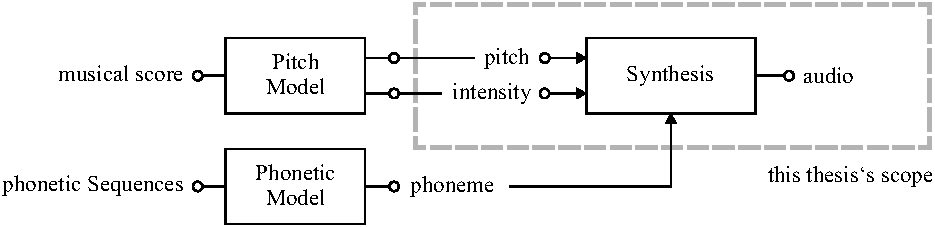
\includegraphics{Graphics/004_thesis_scope.pdf}
    \caption{A text-to-speech singing voice synthesis architecture might consist of a phonetic model, a pitch estimation model and a synthesis model. This thesis scope is limited on the latter.}
    \label{fig:thesis_architecture_scope}
\end{figure}

One possible architecture for a singing voice synthesis model is shown in figure \ref{fig:thesis_architecture_scope}. While the two control parameters pitch and intensity can be controlled directly, they can also be generated from a music score. Phonetic singing voice synthesis methods also include some form of phonetic model, either as a separate component or by conditioning networks using phonemes.\\
In this thesis we want to focus on highly efficient singing voice synthesis, incorporating advances of the past years into classic digital signal processing. To achieve this, this thesis's scope is narrowed down to the synthesis of sung vowels. We therefore do not include a phonetic model or discuss the topic of pitch modelling.
Furthermore, we aim for a multi-singer model, that not only allows voice synthesis using different voice timbre qualities but also morphing between those qualities to create new virtual singers. For analysis, the VocalSet dataset \cite{wilkins_vocalset:_2018} is used to extract pitch and intensity trajectories as well as voice timbre qualities for different virtual singers. This thesis's research questions are as follows:

\begin{itemize}
    \item What methods provide exceptional computational efficiency while still capturing singers voice timbre qualities?
    \item How can we morph efficiently between virtual voices without loosing naturalness?
    \item What validation methods prove suitable for evaluating the naturalness of both synthesized and morphed, synthesized voices.
\end{itemize}

Answering these questions will help us understand important aspects of singing voice synthesis. What might a minimal model for a virtual voice look like that still manages to capture the singers voice qualities? What aspects of a voice are critical for its perception as natural and not synthetic. Application cases for the proposed method can be found in the music software industry. Some scenarios are the implementation of digital choirs or the synthesis of backing or harmonization vocals.\\

With singing voice synthesis being a highly researched topic, the limited scope considered in  this thesis is supposed to help in two ways. Firstly, we aim to differentiate this thesis from existing research. Secondly the limited scope is supposed to reduce the expected workload to a manageable amount, considering the time frame of the thesis of six months and the authors lack of prior knowledge on the topic of singing voice synthesis. \comment{Not sure if this "meta" block is necessary.}
